\section{Potentiale}\label{sec:Potentiale}

\subsection{Definitionen}

\begin{defn}
	Zu einem Spiel $\Gamma = (I, X, (c_i)_{i\in I})$ heißt eine Funktion $P: X \to \IR$
	\begin{itemize}
		\item \emph{verallgemeinertes Nash-Potential}, wenn jedes Minimum von $P$ ein Nash-Gleichgewicht in $\Gamma$ ist, d.h. für alle $x \in X$ gilt:
			\[P(x) = \min_{\hat{x} \in X}P(\hat{x}) \implies \forall i \in I, \hat{x}_i \in X_i: c_i(x) \leq c_i(x \mid \hat{x}_i) \]
		\item \emph{Nash-Potential}, wenn jedes Minimum von $P$ ein Nash-Gleichgewicht in $\Gamma$ ist und umgekehrt, d.h. für alle $x \in X$ gilt:
			\[P(x) = \min_{\hat{x} \in X}P(\hat{x}) \iff \forall i \in I, \hat{x}_i \in X_i: c_i(x) \leq c_i(x \mid \hat{x}_i) \]
		\item \emph{Beste Antwort-Potential}, wenn für jeden Spieler $i$ und alle Strategieprofile $x \in X$ gilt:
			\[\arg\min_{\hat{x}_i \in X_i}c_i(x \mid \hat{x}_i) = \arg \min_{\hat{x}_i \in X_i} P(x \mid \hat{x}_i)\]
		\item \emph{verallgemeinertes ordinales Potential}, wenn für jeden Spieler $i$ und alle Strategieprofile $x \in X$ sowie $\hat{x}_i \in X_i$ gilt:
			\[c_i(x) > c_i(x \mid \hat{x}_i) \implies P(x) > P(x \mid \hat{x}_i)\]
		\item \emph{ordinales Potential}, wenn für jeden Spieler $i$ und alle Strategieprofile $x \in X$ sowie $\hat{x}_i \in X_i$ gilt:
			\[c_i(x) > c_i(x \mid \hat{x}_i) \iff P(x) > P(x \mid \hat{x}_i)\]
		\item \emph{skaliertes Potential}, wenn es streng monotone Funktionen $f_i: \IR \to \IR$ gibt, die $0$ auf $0$ abbilden, sodass für jeden Spieler $i$ und alle Strategieprofile $x \in X$ sowie $\hat{x}_i \in X_i$ gilt:
			\[c_i(x) - c_i(x \mid \hat{x}_i) = f_i(P(x) - P(x \mid \hat{x}_i))\]
		\item \emph{gewichtetes Potential}, wenn es einen Gewichtsvektor $(w_i)_{i\in I} \in \IR_{>0}^I$ gibt, sodass für jeden Spieler $i$ und alle Strategieprofile $x \in X$ sowie $\hat{x}_i \in X_i$ gilt:
			\[c_i(x) - c_i(x \mid \hat{x}_i) = w_i\cdot(P(x) - P(x \mid \hat{x}_i))\]
		\item \emph{exaktes Potential}, wenn für jeden Spieler $i$ und alle Strategieprofile $x \in X$ sowie $\hat{x}_i \in X_i$ gilt:
			\[c_i(x) - c_i(x \mid \hat{x}_i) = P(x) - P(x \mid \hat{x}_i)\]
	\end{itemize}
\end{defn}\todo{Kann man diese Definition irgendwie kompakter/übersichtlicher machen?}

Exakte, gewichtete, ordinale und verallgemeinerte ordinale Potentiale wurden erstmals in \cite{MonShap} definiert, beste Antwort-Potentiale erstmals in \cite{BestRespPot}.

\subsection{Anschauung}

Eine leicht andere Sichtweise auf Potentiale ist, dass diese ein alternatives Koordinationsspiel auf dem Strategieraum des Ausgangsspiels definieren (mit der Potentialfunktion als gemeinsamer Kostenfunktion aller Spieler). In einem solchen Spiel ist es nun viel einfacher beispielsweise Gleichgewichts- oder Optimalitätspunkte zu finden (da hierzu nur eine einzige Funktion betrachtet werden muss). Eigenschaften, die beim Übergang zurück zum ursprünglichen Spiel erhalten bleiben, kann man dann in dem einfacheren Spiel überprüfen. Diesen Übergang werden wir später mit Hilfe von (Iso-)Morphismen formal fassen (siehe \Cref{sec:Morphismen}).

Hier wollen wir nun noch kurz darauf eingehen, wie sich die verschiedenen Potentialbegriffe anschaulich voneinander unterscheiden. Wir betrachten dazu (endliche) 2-Personenspiele. Deren Strategieraum kann man dann als Gitternetz in der Ebene auffassen, wobei jede Strategie von Spieler 1 einer senkrechten und jede Strategie von Spieler 2 einer waagerechten Gitterlinie entspricht. Kreuzungspunkte von zwei Gerade entsprechen dann gerade vollständige Strategieprofilen. Kostenfunktionen (ebenso wie Potentiale) sind dann \glqq Reliefkarten\grqq{}, deren Höhe den jeweiligen Kosten entspricht. 

\begin{figure}[h]\centering
	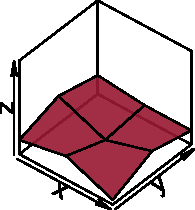
\includegraphics[width=.3\textwidth]{../Bilder/exaktesPotentialSp1.pdf}
	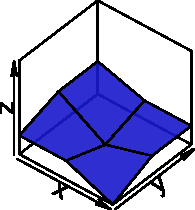
\includegraphics[width=.3\textwidth]{../Bilder/exaktesPotentialSp2.pdf}
	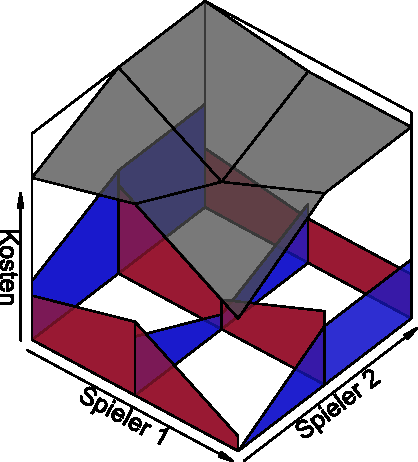
\includegraphics[width=.3\textwidth]{../Bilder/exaktesPotential.pdf}
	\caption{Ein 2-Personenspiel mit exaktem Potential (grau): Spieler 1: rot, Spieler 2: blau}
\end{figure}

Ein exaktes Potential entspricht in diesem Bild einer gemeinsamen Reliefkarte für beide Spieler, die - im Falle eines exakten Potentials - \glqq scheibenweise\grqq{} bis auf eine additive Konstante mit der eigentlichen Kostenfunktion übereinstimmt. Anders formuliert: Wird die Strategie eines Spieler festgehalten, so kann der andere Spieler seine Kostenveränderungen bei der Wahl der verschiedenen ihm zur Verfügung stehenden Strategien auch anhand der Potentialfunktion ablesen. 

Geht man nun über zu einem gewichteten Potential, so lesen die beiden Spieler das Potential sozusagen in verschiedenen Einheiten\todo{eigentlich müssen verchiedene Einheiten nicht zwangsläufig proportional zueinander sein - für Längeneinheiten sollte es typischerweise aber stimmen}. Das heißt die Kostenveränderungen eines Spielers sind nur noch proportional zu den Potentialänderungen. Ein skaliertes Potential zeigt jedem Spieler noch an, welche der Kostenveränderungen eher groß und welche klein sind. Ordinale Potentiale zeigen nur noch die Richtung der Kostenveränderung an (\glqq wird teurer\grqq / \glqq wird billiger\grqq / \glqq Kosten bleiben konstant\grqq) und verallgemeinerte ordinale Potentiale zeigen nur noch echte Steigungen korrekt an. Beste-Antwort-Potentiale schließlich zeigen immer die beste Antwort an.


\todo[inline]{Zusammenhänge (evtl. schon nächstes Kapitel?)}

Eine Beobachtung aus \cite{CharExGewPotinWCG}:

\begin{beob}\label{beob:ZshExGewPot}
	Ein Spiel $\Gamma = (I, (X_i)_{i \in I}, (c_i)_{i \in I})$ besitzt genau dann ein gewichtetes Potential (mit Gewichtsvektor $(w_i)_{i \in I}$), wenn $\Gamma' := (I, (X_i)_{i \in I}, (w_i \cdot c_i)_{i \in I})$ ein exaktes Potential besitzt.
\end{beob}

Folgt auch aus einer allgemeineren Beobachtung in \Cref{sec:Morphismen}.

\subsection{Erste Sätze}

Zu einem gegebenen Strategieprofil $x \in X$ sei dessen \emph{Nachbarschaft} die Menge aller durch höchstens eine Abweichung erreichbarer Strategieprofile, d.h. die Menge $\{(\hat{x}_i, x_{-i}) | i \in N, \hat{x}_i \in X_i\}$. Wir nennen $x$ dann ein \emph{lokales Minimum} einer Funktion $f: X \to \IR$, wenn es ein Minimum innerhalb seiner Nachbarschaft ist.

\begin{satz}\label{satz:lokMinNG}
	Sei $\Gamma$ ein Spiel mit einem verallgemeinerten ordinalen Potential $P$. Dann ist jedes lokale Minimum von $P$ ein Nash-Gleichgewicht von $\Gamma$. Ist $P$ sogar ein ordinales Potential, so gilt auch die umgekehrte Richtung.
\end{satz}

\todo[inline]{Diese Sätze hier evtl. nur erwähnen und erst später (nach der Definition von Morphismen) formalisieren (und beweisen)}

Dieser Satz zeigt also, dass man Nash-Gleichgewichte allein durch Betrachten einer Potentialfunktion finden kann. Daraus  folgt direkt die Existenz von Nash-Gleichgewichten in einer Vielzahl von Potentialspielen:

\begin{kor}
	Sei $\Gamma$ ein Spiel mit einem kompakten Strategieraum und einer stetigen verallgemeinerten ordinalen Potentialfunktion. Dann hat $\Gamma$ wenigstens ein Nash-Gleichgewicht.
\end{kor}

Insbesondere also haben endliche Potentialspiele immer ein Nashgleichgewicht. \Cref{satz:lokMinNG} folgt mit Hilfe von \Cref{kor:ExVerbPfadExNG} direkt aus dem folgenden Satz\todo{Streng genommen nicht wirklich, da das Korollar nur für Spiele gilt!?}:

\begin{satz}
	Sei $\Gamma$ ein Spiel mit einem verallgemeinerten ordinalen Potential $P$. Dann ist jeder Verbesserungspfad in $\Gamma$ auch ein Verbesserungspfad bezüglich $P$. Ist $P$ sogar ein ordinales Potential, so gilt auch die umgekehrte Richtung.
\end{satz}

\begin{proof}.
	
	\todo[inline]{Beweis}	
\end{proof}

\todo[inline]{Was kann man über Beste-Antwort-Potentiale sagen (vermtl. Zusammenhang zu Beste-Antwort-Pfade?)}

Für Spiele mit unendlicher Spielermenge erweist es sich als hilfreiche Beobachtung, dass wir Potentiale pfadzusammenhangskomponentenweise definieren können:

\begin{beob}\label{beob:KompWeisePotentiale}
	Sei $\Gamma$ ein beliebiges Spiel und $P: X \to \IR$ eine Funktion. Erfüllt $P$ dann die Bedingung eines exakten/gewichteten/skalierten/ordinalen/verallgemeinerten ordinalen Potentials für jede (maximale) Pfadzusammenhangskomponente, so ist $P$ ein entsprechendes Potential für ganz $\Gamma$.
\end{beob}

\begin{proof}
	Dies folgt direkt aus dem Umstand, dass die definierende Eigenschaft für alle aufgezählten Potentiale immer nur entlang eines Pfades (der Länge $1$) und damit innerhalb einer Zusammenhangskomponente geprüft werden muss.
\end{proof}

\subsection{Charakterisierungen der Potentiale}

\begin{satz}\label{satz:CharExPot}
	Ein Spiel besitzt genau dann ein exaktes Potential, wenn alle 4-Zykel im Strategieraum eine Gesamtänderung von $0$ haben.
\end{satz}

\begin{proof}
	Wir folgen dem Beweis aus \cite[Anhang A]{MonShap}. Dort wird der Satz zwar nur für $N$-Personenspiele gezeigt, mit \Cref{beob:KompWeisePotentiale} überträgt sich dieser Beweis aber direkt auch auf allgemeine Spiele.
	
	Sei zunächst $\gamma \coloneqq (x^0, x^1, x^2, x^3, x^4)$ ein beliebiger 4-Zykel in einem Spiel mit Potential $P$. Dann gilt für die Gesamtänderung:
		\[\delta(\gamma) = \sum_{i=0}^3 \left(c_{i(k)}(x^{k+1}) - c_{i(k)}(x^k)\right) = \sum_{k=0}^{3} \left(P(x^{k+1}) - P(x^k)\right) = P(x^4) - P(x^0) = 0^{}\]
		
	Ist umgekehrt $\Gamma$ ein Spiel, in dem für alle 4-Zykel $\gamma$ gilt $\PfadAend(\gamma) = 0$, $x$ ein beliebiges, aber festes Strategieprofil in $\Gamma$ und $Y_x$ dessen Pfadzusammenhangskomponente, dann definiere wie folgt eine Funktion $P_x$ auf $Y_x$:
		\[P: Y_x \to \IR: y \mapsto \PfadAend(\gamma), \,\gamma \text{ beliebiger Pfad von } x \text{ nach } y \]
	Damit diese Funktion tatsächlich wohldefiniert ist, muss für je zwei Pfade $\gamma$ und $\gamma'$ von $\hat{x}$ nach $x$ gelten, dass die jeweiligen Gesamtänderungen gleich sind, d.h. $\PfadAend(\gamma) = \PfadAend(\gamma')$. Dies ist äquivalent dazu, dass der Zykel, den man durch Verknüpfen der beiden Pfade $\gamma$ und $\overset{\leftarrow}{\gamma'}$ erhält eine Gesamtänderung von $0$ hat. Dazu zeigen wir nun mittels Induktion über deren Länge, dass für alle Zykel $\mu$ gilt $\PfadAend(\mu) = 0$:
	\begin{description}
		\item[IA ($\bm{\abs{\mu}=4}$)\footnote{Zykel der Längen $0$, $2$ und $3$ haben automatisch immer Gesamtänderung $0$, da in ihnen alle Abweichungen vom gleichen Spieler vorgenommen werden müssen.}] D.h. $\mu$ ist ein 4-Zykel und damit $\PfadAend(\mu) = 0$ nach Voraussetzung.
		\item[IS ($\bm{\abs{\mu}\eqqcolon n}$)] Vorausgesetzt es gibt einen Pfad $\mu' = (x'^0, \dots, x'^n)$ gleicher Länge und Gesamtänderung wie $\mu$, sodass in den ersten beiden Schritten der gleiche Spieler seine Strategie wechselt, d.h. $i(0)=i(1)$. Dann erhält man durch Weglassen des ersten Schrittes einen \emph{kürzeren} Pfad $\mu'' \coloneqq (x'^0, x'^2, \dots, x'^n)$ mit gleicher Gesamtänderung, welche dann nach Induktion bereits $0$ ist. Indiesem Fall haben wir dann wie gewünscht $\PfadAend(\mu) = \PfadAend(\mu') = \PfadAend(\mu'') = 0$.
		
		Die Existenz eines solchen Pfades $\mu'$ zeigen wir nun mittels Induktion über $k \coloneqq min\left\{1 \leq l < n \setMid i(l) = i(0)\right\}$. Ein solches $k$ existiert immer, da Spieler $i(0)$ bereits im ersten Schritt seine Strategie wechselt und dies daher im Verlauf des Zykels noch mindestens ein weiteres Mal tun muss.
		\begin{description}
			\item[IA ($\bm{k=1}$)] Dann gilt bereits $i(0)=i(1)$ und wir sind fertig mit $\mu' \coloneqq \mu$.
			\item[IS ($\bm{k-1\to k}$)] Wir ändern $\mu$ so ab, dass Spieler $i(0)$ bereits im $(k-1)$-ten Schritt der abweichende Spieler ist. Dann sind wir fertig nach Induktionsvoraussetzung. Dazu ersetzen wir in $\mu$ das Strategieprofil $x^k$ durch $(x^{k-1} \mid x^{k+1}_{i(0)})$, sodass also Spieler $i(0)$ bereits einen Schritt früher (im $(k-1)$-ten) seine Strategie wechselt und der Spieler, der dies zuvor in diesem Schritt getan hat, einen Schritt später.
			
			Bei dieser Anpassung bleibt die Gesamtänderung des Pfades $\mu$ gleich, denn wir ersetzen lediglich ein Pfadstück der Länge $2$ durch ein anderes Pfadstück der Länge $2$. Und da sich diese beiden Pfade zu einem 4-Zykel zusammensetzen lassen, haben diese nach Voraussetzung die gleiche Gesamtänderung.
			
			Auf dieses abgeänderte $\mu$ können wir nun die Induktionsvoraussetzung anwenden und erhalten dadurch einen neuen Pfad $\mu'$ mit den gewünschten Eigenschaften.
		\end{description}
		Hiermit können wir auch den Induktionsschritt der äußeren Induktion und damit den Nachweis der Wohldefiniertheit von $P$ abschließen. 
	\end{description}	
	Wählen wir nun für jede maximale Pfadzusammenhangskomponente ein einziges $x$ in dieser und definieren wie oben eine Funktion $P_x$, so lassen sich alle diese Funktionen zu einer Funktion $P$ auf ganz $X$ zusammensetzen. Nach Definition erfüllt diese auf jeder Pfadzusammenhangskomponente die Bedingung eines exakten Potentials. Also ist nach \Cref{beob:KompWeisePotentiale} $P$ ein exaktes Potential auf $X$.
\end{proof}

\begin{satz}\label{satz:CharGewPot}
	Ein Spiel besitzt genau dann ein gewichtetes Potential, wenn ... \todo{analoge Bedingung zu exaktem Potential (vgl. \cite[Kapitel 3.2]{CharExGewPotinWCG})}
\end{satz}

\begin{proof}.
	
	\todo[inline]{mit \Cref{beob:ZshExGewPot}?}
\end{proof}

\todo[inline]{Charakterisierung der Existenz eines skalierten Potentials?}

\begin{defn}
	Eine Menge $X$ mit einer strikten Partialordnung $\prec$ (irreflexiv und transitiv) heißt \emph{reell geordnet}\footnote{\citeauthor{CharExOrdPot} bezeichnen solche Mengen in \cite{CharExOrdPot} als \glqq properly ordered\grqq}, wenn es eine strikt monotone Abbildung von $X$ in die reellen Zahlen gib, also $f: X \to \IR$ mit $x \prec x' \implies f(x) < f(x')$.
\end{defn}

Wir definieren nun eine Äquivalenzrelation auf dem Strategieraum:\todo{evtl. schon im Grundlagenkapitel gemeinsam mit Pfadzusammenhangskomponenten?}
	\[x \NVrel y \dIff \text{ es gibt einen nicht-Verschlechterungspfad von $x$ nach $y$ und umgekehrt}\]
Auf dem dadurch erzeugten Raum von Äquivalenzklassen $\XmodNV \coloneqq \left\lbrace[x] \mid x \in X\right\rbrace$ erhält man eine transitive Ordnung
	\[[x] \SVord [y] \dIff \text{Es gibt einen schwachen Verbesserungspfad von $y$ nach $x$}\]
Sowohl Wohldefiniertheit als auch Transitivität dieser Relation ergeben sich aus der Beobachtung, dass die Verknüpfung eines nicht-Verschlechterungspfades mit einem schwachen Verbesserungspfad wieder einen schwachen Verbesserungspfad ergibt.

Damit zeigen \citeauthor{CharExOrdPot} in \cite[Theorem 3.1]{CharExOrdPot} folgende Charakterisierung der Existenz von ordinalen Potentialen:

\begin{satz}\label{satz:CharOrdPot}
	Ein Spiel besitzt genau dann ein ordinales Potential, wenn es keine schwachen Verbesserungszykel enthält und $(\XmodNV, \SVord)$ reell geordnet ist.
\end{satz}

\begin{proof}
	Sei zunächst $P: X \to \IR$ ein ordinales Potential eines Spiels $\Gamma$. Dann gilt:
	\begin{enumerate}
		\item $\Gamma$ enthält keine schwachen Verbesserungszykel. Denn angenommen $\gamma = (x^0, \dots, x^n)$ wäre ein schwacher Verbesserungszykel in $\Gamma$, so gilt für alle $0 \leq k < n$: $c_{i(k)}(x^{k+1}) \leq c_{i(k)}(x^k)$ und für ein solches $k$ sogar $c_{i(k)}(x^{k+1}) < c_{i(k)}(x^k)$. Da ferner $P$ ein ordinales Potential ist, folgt daraus:
			\[P(x^0) \leq P(x^1) \leq \dots \leq P(x^{k+1}) < P(x^k) \leq \dots \leq P(x^n) = P(x^0)\]
		Dies ist jedoch ein Widerspruch. Also kann es keinen solchen Verbesserungszykel geben.
		
		\item $\SVord$ ist eine strikte Partialordnung auf $\XmodNV$. Denn die Relation ist immer transitiv und in der Abwesenheit von schwachen Verbesserungszykeln zudem irreflexiv. Gäbe es nämlich ein Strategieprofil mit $[x] \SVord [x]$, so gäbe es einen schwachen Verbesserungspfad von $x$ nach $x$, also einen schwachen Verbesserungszykel.
		
		\item $(\XmodNV, \SVord)$ ist reell geordnet. Definiere dazu die Abbildung $f: \XmodNV \to \IR: [x] \mapsto P(x)$. Diese ist wohldefiniert, denn ist $y \in [x]$, so gibt es also Nichtverschlechterungspfade von $x$ nach $y$ und umgekehrt. Zusammen bilden dieses einen Nichtverschlechterungszykel und da es keine schwachen Verbesserungszykel in $\Gamma$ gibt, muss in die diesem Zykel (und damit bereits in den beiden Pfaden) in jedem Schritt Gleichheit gelten. Insbesondere folgt damit $P(x) = P(y)$.
		
		Ferner ist diese Abbildung streng monoton, denn gilt $[x] \SVord [y]$, so gibt es einen schwachen Verbesserungspfad $\gamma$ von $y$ nach $x$. Damit folgt analog zum ersten Punkt: $P(x) < P(y)$
	\end{enumerate}

	Ist umgekehrt $\Gamma$ ein Spiel ohne schwache Verbesserungszykel, so ist - wie bereits gezeigt - $\SVord$ eine strikte Partialordnung auf $\XmodNV$. Sei nun $(\XmodNV, \SVord)$ sogar reell-geordnet mit Abbildung $f: \XmodNV \to \IR$, so definiere $P: X \to \IR: x \mapsto f([x])$. Dies ist ein ordinales Potential, denn es gilt:
	\begin{enumerate}
		\item Gilt $c_i(x) > c_i(x \mid \hat{x}_i)$, so ist $(x, (x \mid \hat{x}_i))$ ein schwacher Verbesserungspfad. Da es in $\Gamma$ keine schwachen Verbesserungszykel gibt, kann es also keinen nicht-Verschlechterungspfad in die andere Richtung geben und es gilt: $[x] \succ [(x \mid \hat{x}_i)]$. Daraus wiederum folgt $P(x) = f([x]) > f([(x \mid \hat{x}_i)]) = P(x \mid \hat{x}_i)$.
		\item Gilt $c_i(x) = c_i(x \mid \hat{x}_i)$, so sind sowohl $(x, (x \mid \hat{x}_i))$ als auch $((x \mid \hat{x}_i), x)$ nicht-Verschlechterungspfade, also $[x] = [(x \mid \hat{x}_i)]$ und damit $P(x) = f([x]) = f([(x \mid \hat{x}_i)]) = P(x \mid \hat{x}_i)$. \qedhere
	\end{enumerate}
\end{proof}

\begin{bem}
	Im Gegensatz zur Charakterisierung von exakten Potentialspielen in \Cref{satz:CharExPot} genügt es für die Existenz eines ordinalen Potentials nicht, nur Zykel der Länge 4 zu betrachten. \citeauthor{CharExOrdPot} geben dafür in \cite[Beispiel 3.1]{CharExOrdPot} ein Gegenbeispiel mit zwei Spielern und je drei Strategien an.
\end{bem}

Anlehnend an \Cref{satz:CharOrdPot} erhält man unter Verwendung der Relation
	\[x \VerbRel y \dIff \text{ es gibt einen Verbesserungspfad der Länge $\geq 1$ von $y$ nach $x$}\]
eine Charakterisierung der Existenz eines verallgemeinerten ordinalen Potentials:
\begin{satz}\label{satz:CharVerallOrdPot}
	Ein Spiel besitzt genau dann ein verallgemeinertes ordinales Potential, wenn $(X, \VerbRel)$ reell geordnet ist.
\end{satz}

\begin{proof}
	$(X, \VerbRel)$ reell geordnet mit streng monotoner Abbildung $f: X \to \IR$, so sieht man direkt, dass $f$ auch ein verallgemeinertes Potential ist. Denn für $x \in X, \hat{x}_i \in X_i$ mit $c_i(x) > c_i(x \mid \hat{x}_i)$ ist $(x, (x \mid \hat{x}_i))$ ein Verbesserungspfad, also $(x \mid \hat{x}_i) \VerbRel x$ und damit $f(x \mid \hat{x}_i) < f(x)$.
	
	Haben wir hingegen ein Spiel $\Gamma$ mit einem verallgemeinerten ordinalen Potential $P$, so ist $(X, \VerbRel)$ reell geordnet, denn
	\begin{enumerate}
		\item $\VerbRel$ ist eine strikte Partialordnung auf $X$: Sie ist transitiv, da die Verknüpfung zweier Verbesserungspfade wieder ein Verbesserungspfad ist, und irreflexiv, da es in $\Gamma$keine Verbesserungszykel gibt. Angenommen nämlich $\Gamma$ enthielte einen solchen Verbesserungszykel $\gamma = (x^0, \dots, x^n)$, d.h. für alle $0 \leq k < n$ gilt $c_{i(k)}(x^{k+1}) < c_{i(k)}(x^k)$. Da $P$ ein verallgemeinertes ordinales Potential ist, folgt daraus $P(x^0) > P(x^1) > \dots > P(x^n) = P(x^0)$, ein Widerspruch. Also kann es keinen Verbesserungszykel geben und damit nie $x \VerbRel x$ gelten.
		\item $(X, \VerbRel)$ ist reell geordnet durch die Funktion $P: X \to \IR$. Gilt nämlich $x \VerbRel y$, so gibt es also einen Verbesserungspfad von $y$ nach $x$. Da $P$ ein verallgemeinertes ordinales Potential ist, nimmt es entlang dieses Pfades in jedem Schritt ab, und folglich gilt $P(y) > P(x)$. Damit ist $P$ streng monoton auf $(X, \VerbRel)$. \qedhere
	\end{enumerate} 
\end{proof}

In dieser Form ist dies noch eine wenig hilfreiche Charakterisierung, denn um zu zeigen, dass der Strategieraum reell geordnet ist, muss man effektiv bereits die Potentialfunktion angeben. Allerdings erhält man daraus mit Hilfe der folgenden Propositionen einfachere Charakterisierungen für gewisse Teilklassen von Spielen:

\begin{prop}\label{prop:AbzReellGeordnet}
	Jede abzählbare Menge mit einer strikten Partialordnung ist bereits reell geordnet.
\end{prop}

Ein Beweis dazu findet sich in \cite[Lemma 2.2]{CharExOrdPot}. Noch allgemeiner zeigen\todo{wirklich gezeigt wird es dort eigentlich nicht (sondern auf andere Quelle verwiesen)}{} \citeauthor{CharExOrdPot}, dass es sogar genügt, wenn die partiell geordnete Menge eine bezüglich dieser Ordnung dichte, abzählbare Teilmenge hat.

\begin{prop}\label{prop:VerRelPartOrdVerbz}
	Die Relation $\VerbRel$ ist genau dann eine strikte Partialordnung, wenn $\Gamma$ keine Verbesserungszykel enthält.
\end{prop}

\begin{proof}
	Da die Verknüpfung eines Verbesserungspfades von $z$ nach $y$ mit einem von $y$ nach $x$ einen Verbesserungspfad von $z$ nach $z$ ergibt, ist $\VerbRel$ automatisch immer transitiv.
	
	Ferner ist $\VerbRel$ genau dann irreflexiv, wenn für alle $x \in X$ gilt, dass $x \not\VerbRel x$, es also keinen Verbesserungspfad von $x$ nach $x$ gibt. Und letzteres entspricht genau einem (bei $x$ beginnenden) Verbesserungskreis.
\end{proof}

\begin{kor}\label{kor:CharExVerOrdPotabzX}
	Ein Spiel mit abzählbarem Strategieraum besitzt genau dann ein verallgemeinertes ordinales Potential, wenn es keine Verbesserungskreise enthält.
\end{kor}

\begin{proof}
	Nach \Cref{prop:AbzReellGeordnet} ist jede abzählbare Menge mit einer strikten Partialordnung bereits reell geordnet. Also macht $\VerbRel$ einen abzählbaren Strategieraum genau dann zu einer reell geordneten Menge, wenn $\VerbRel$ eine strikte Partialordnung ist. Und dies ist nach \Cref{prop:VerRelPartOrdVerbz} genau dann der Fall, wenn das Spiel keine Verbesserungszykel enthält.
\end{proof}

Laut \Cref{beob:KompWeisePotentiale} gilt diese Charakterisierung sogar für die größere Klasse der Spiele mit abzählbar großen Pfadzusammenhangskomponenten. Insbesondere gilt damit:

\begin{kor}
	Ein Spiel mit abzählbar vielen Spielern und abzählbar großen spielerspezifischen Strategieräumen besitzt genau dann ein verallgemeinertes ordinales Potential, wenn es keine Verbesserungskreise enthält.
\end{kor}

\begin{proof}
	Wir müssen zeigen, dass in einem solchen Spiel jede Pfadzusammenhangskomponente abzählbar groß ist. Seien dazu also $x \in X$ und $n \in \INs$ beliebig. Dann ist
		\[Y_x^n \coloneqq \left\{y \in X \setMid \exists \gamma \text{ Pfad der Länge $n$ von $x$ nach $y$}\right\}, \]
	die Menge aller von $x$ aus durch Pfade der Länge $n$ erreichbaren Strategieprofile, abzählbar. Denn es gilt induktiv:
	\begin{description}
		\item[IA ($\bm{n=1}$)] Es ist
			\[Y_x^1 = \left\{y \in X \setMid \exists i \in I: y = (x \mid y_i)\right\} = \left\{(x \mid y_i) \setMid i \in I, y_i \in Y_i \right\} = \bigcup_{i \in I} \left\{(x \mid y_i) \setMid y_i \in Y_i \right\}\]
			eine abzählbare Vereinigung (da die Spielermenge abzählbar ist) von abzählbar großen Mengen (den spielerspezifischen Strategieräumen), also selbst abzählbar groß.
		\item[IS ($\bm{<n \to n}$)] Es ist
			\[Y_x^n = \bigcup_{y \in Y_x^{n-1}} Y_y^1\]
			eine (nach Induktionsvoraussetung) abzählbare Vereinigung abzählbar großer Mengen und daher selbst wieder abzählbar.
	\end{description}
	Folglich ist auch $Y_x = \bigcup_{n\in\INs} Y_x^n$ abzählbar und besitzt folglich nach \Cref{kor:CharExVerOrdPotabzX} ein verallgemeinertes ordinales Potential.
\end{proof}

Beschränkt man sich hingegen auf die kleinere Klasse von endlichen Spielen, so erhält man die (auf anderem Wege) erstmals von \citeauthor{MonShap} in \cite[Lemma 2.5]{MonShap} gezeigte Charakterisierung der Existenz von verallgemeinerten ordinalen Potentialen:

\begin{kor}
	Ein endliches Spiel besitzt genau dann ein verallgemeinertes ordinales Potential, wenn es die FIP besitzt.
\end{kor}

\begin{proof}
	In einem Spiel mit endlichem Strategieraum sind unendliche Verbesserungspfade genau die Verbesserungskreise. Damit folgt die Aussage direkt aus \Cref{kor:CharExVerOrdPotabzX}.
\end{proof}

\begin{bem}
	Möchte man in den oben beschriebenen Fällen eine konkrete Potentialfunktion angeben, so kann man dies analog zu einer alternativen, konstruktiven Beweisidee für endliche Spiele aus \cite[Abschnitt 5]{CongGamesPlayerSpecPayoff} tun:

Sei dazu $\Gamma$ ein Spiel mit abzählbarem Strategieraum $X := \{x^1, x^2, \dots \}$ und ohne Verbesserungszykel. Definiere die Funktion $h: X \to \IR: x^k \mapsto 2^{-k}$ sowie für jedes Strategieprofil $x \in X$ die Menge $Y_{>x} \coloneqq \left\{y \in X \setMid \exists \text{ Verbesserungspfad von } y \text{ nach } x\right\}$ und mit deren Hilfe
	\[P: X \to \IR: x \mapsto 1 - \sum_{y \in Y_{>x}} h(y)\]
\end{bem}

\begin{proof}
	Diese Funktion ist wohldefiniert, da $\sum_{k=1}^{\infty} 2^{-k} = 1$ absolut konvergiert. Sie ist außerdem ein verallgemeinertes ordinales Potential, denn gilt $c_i(x) > c_i(x \mid \hat{x}_i)$ so ist $(x, (x \mid \hat{x}_i))$ ein Verbesserungspfad. Außerdem gilt $x \notin Y_{>x}$, da es in $\Gamma$ keine Verbesserungszykel gibt. Damit folgt:
		\[P(x) = 1 - \sum_{y \in Y_{>x}} h(y) > 1 - \sum_{y \in Y_{>x}} h(y) - h(x) = 1 - \sum_{y \in Y_{>(x \mid \hat{x}_i)}}h(y) = P(x \mid \hat{x}_i)\qedhere\]
\end{proof}


Ebenfalls analog zur Charakterisierung für ordinale Potentiale zeigt \citeauthor{BestRespPot} in \cite[Theorem 3.1]{BestRespPot} eine solche für Beste Antwort-Potentiale. Dazu definiert man die Äquivalenzrelation:
	\[x \BArel y \dIff \text{ es gibt einen Beste Antwort-Pfad von $x$ nach $y$ und umgekehrt}\]
und auf dem dadurch erzeugten Raum von Äquivalenzklassen $\XmodBA \coloneqq \left\lbrace[x] \mid x \in X\right\rbrace$ erhält man eine transitive Ordnung
\[[x] \BAord [y] \dIff \text{Es gibt einen schwachen Beste Antwort-Verbesserungspfad von $y$ nach $x$}\]

\begin{satz}
	Ein Spiel besitzt genau dann ein beste Antwort-Potential, wenn es keine schwachen Beste Antwort-Verbesserungszykel enthält und $(\XmodBA, \BAord)$ reell geordnet ist.
\end{satz}

\begin{proof}
	Sei zunächst $P: X \to \IR$ ein beste Antwort-Potential eines Spiels $\Gamma$. Dann gilt:
	\begin{enumerate}
		\item $\Gamma$ enthält keine schwachen Beste Antwort-Verbesserungszykel. Denn angenommen $\gamma = (x^0, \dots, x^n)$ wäre ein schwacher Beste Antwort-Verbesserungszykel in $\Gamma$, so gilt für alle $0 \leq k < n$:
			\[c_{i(k)}(x^{k+1}) = \min_{\hat{x}_{i(k)} \in X_{i(k)}} c_{i(k)}(x^k \mid \hat{x}_i) \leq c_{i(k)}(x^k)\]
		und, da $P$ ein beste Antwort-Potential ist, ebenso 
			\[P(x^{k+1}) = \min_{\hat{x}_{i(k)} \in X_{i(k)}} P(x^k \mid \hat{x}_i) \leq P(x^k).\]
		Ferner gilt für ein solches $k$ sogar $c_{i(k)}(x^{k+1}) < c_{i(k)}(x^k)$, also auch $P(x^{k+1}) < P(x^k)$ (da $x^k_{i(k)}$ keine beste Antwort auf $x^k$ ist). Zusammen folgt daher
			\[P(x^0) \leq P(x^1) \leq \dots \leq P(x^{k+1}) < P(x^k) \leq \dots \leq P(x^n) = P(x^0).\]
		Dies ist jedoch ein Widerspruch. Also kann es keinen solchen Verbesserungszykel geben.
		
		\item $\BAord$ ist eine strikte Partialordnung auf $\XmodBA$. Denn die Relation ist immer transitiv und in der Abwesenheit von schwachen Beste Antwort-Verbesserungszykeln zudem irreflexiv. Gäbe es nämlich ein Strategieprofil mit $[x] \BAord [x]$, so gäbe es einen schwachen Beste Antwort-Verbesserungspfad von $x$ nach $x$, also einen schwachen Beste Antwort-Verbesserungszykel.
		
		\item $(\XmodBA, \BAord)$ ist reell geordnet. Definiere dazu die Abbildung $f: \XmodBA \to \IR: [x] \mapsto P(x)$. Diese ist wohldefiniert, denn ist $y \in [x]$, so gibt es also Beste Antwort-Pfade von $x$ nach $y$ und umgekehrt. Zusammen bilden dieses einen Beste Antwort-Zykel und da es keine schwachen Beste Antwort-Verbesserungszykel in $\Gamma$ gibt, muss in die diesem Zykel (und damit bereits in den beiden Pfaden) in jedem Schritt Gleichheit gelten. Insbesondere folgt damit $P(x) = P(y)$.
		
		Ferner ist diese Abbildung streng monoton, denn gilt $[x] \SVord [y]$, so gibt es einen schwachen Beste Antwort-Verbesserungspfad $\gamma$ von $y$ nach $x$. Damit folgt analog zum ersten Punkt: $P(x) < P(y)$
	\end{enumerate}
	
	Ist umgekehrt $\Gamma$ ein Spiel ohne schwache Beste Antwort-Verbesserungszykel, so ist - wie bereits gezeigt - $\BAord$ eine strikte Partialordnung auf $\XmodBA$. Sei nun $(\XmodBA, \BAord)$ sogar reell-geordnet mit Abbildung $f: \XmodBA \to \IR$, so definiere $P: X \to \IR: x \mapsto f([x])$. Dies ist ein beste Antwort-Potential, denn es gilt $\arg \min_{x'_i \in X_i}c_i(x \mid x'_i) = \arg \min_{x'_i \in X_i} P(x \mid x'_i)$:
	\begin{description}
		\item[\glqq$\bm{\subseteq}$\grqq:] Ist $\hat{x}_i \in \arg \min_{\hat{x}_i \in X_i}c_i(x \mid \hat{x})$, so ist also $\hat{x}_i$ insbesondere auch eine beste Antwort auf alle Strategieprofile $(x \mid x'_i)$ für $x'_i \in X_i$.
			\begin{description}
				\item[1. Fall:] Gilt $c_i(x \mid \hat{x}_i) < c_i(x \mid x'_i)$, so ist $((x \mid x'_i), (x \mid \hat{x}_i))$ ein Beste Antwort-Verbesserungspfad, also $[(x \mid \hat{x}_i)] \BAord [(x \mid x'_i)]$ und damit $P(x \mid \hat{x}_i) = f([(x \mid \hat{x}_i)]) < f ([(x \mid x'_i)]) = P(x \mid x'_i)$.
				\item[2. Fall:] Gilt $c_i(x \mid \hat{x}_i) = c_i(x \mid x'_i)$, so sind sowohl $((x \mid x'_i), (x \mid \hat{x}_i))$ als auch $((x \mid \hat{x}_i), (x \mid x'_i))$ Beste Antwort-Pfade und folglich $(x \mid x'_i) \BArel (x \mid \hat{x}_i)$. Somit folgt $P(x \mid \hat{x}_i) = f([(x \mid \hat{x}_i)]) = f([(x \mid x'_i)]) = P(x \mid x'_i)$.
			\end{description}
			Insgesamt gilt also für alle $x'_i \in X_i$, dass $P(x \mid \hat{x}_i) \leq P(x \mid x'_i)$ und daher $\hat{x}_i \in \arg \min_{x'_i \in X_i} P(x \mid x'_i)$.
		\item[\glqq$\bm{\supseteq}$\grqq:] .
		
		\todo[inline]{Funktioniert dieser Beweis an der Stelle überhaupt? }
	\end{description}
\end{proof}

\todo[inline]{vgl. mit \cite{BestRespPot}, evtl. weglassen?}


Die Existenz eines verallgemeinerten Nash-Potentials schließlich lässt sich für endliche Spiele trivialerweise dadurch charakterisieren, dass das entsprechende Spiel ein Nash-Gleichgewicht besitzt. Hat nämlich ein Spiel $\Gamma$ mindestens ein Nash-Gleichgewicht, so ist die Funktion
	\[P: X \to \IR: x \mapsto \begin{cases}0, &x \text{ ist ein Nash-Gleichgewicht} \\ 1, &x \text{ ist kein Nash-Gleichgewicht}\end{cases} \]
ein verallgemeinertes Nash-Potential (das sogar alle Nash-Gleichgewichte auszeichnet).

Umgekehrt kann ein endliches Spiel ohne Nash-Gleichgewichte nie ein verallgemeinertes Nash-Potential besitzen, da jede Funktion auf dem endlichen Strategieraum $X$ mindestens ein Minimum besitzt (welches also einem Nash-Gleichgewicht entsprechen müsste).

Spiele mit unendlichem Strategieraum besitzen immer verallgemeinerte Nash-Potentiale, nämlich zumindest alle Funktionen, welche kein Minimum besitzen.
	